\subsection{Questão de Investigação 2}
A segunda questão de investigação trata-se de saber se \textbf{existe alguma diferença significativa na taxa de cobertura dos testes, nos grupos com duas e quatro pessoas}. Para o estudo dessa métrica, analisou-se o ficheiro Excel e verificou-se que se deveria usar a variável M2(Número de técnicos no projeto de ESII) e M24 (Taxa de cobertura de código), que são variáveis independentes. Apenas vai ser analisado para grupos de duas e quatro pessoas, pois um grupo só pode ter no máximo quatro elementos, e não pode haver grupos com apenas um elemento, e como não existiram grupos com três elementos, apenas vai ser realizado este estudo para os grupos de dois e quatros elementos.

\vspace{0.2cm}


Após essa verificação percebemos que deveria de ser usado um teste de localização. Após essa conclusão, foram separadas as amostras das taxas de cobertura dos grupos com dois elementos e dos grupos com quatro elementos, fez-se o tratamento de outliers especificado e removeu-se os dados da primeira recolha, pois ainda não se tinha começado a escrever código nessa recolha, logo a taxa de cobertura dos testes iria ser sempre zero, sendo redundante para a pesquisa que se quer realizar. 


\vspace{0.2cm}
Para a análise das variáveis, realizou-se um summary para cada variável e um boxplot, como pode ser visto nas Figuras \ref{summary_2elementos}, \ref{summary_4elementos} e \ref{boxplotGruposquestao2}.


\begin{figure}
    \centering
    \caption{Summary da taxa de cobertura dos grupos com dois elementos}
    \includegraphics[width=0.5\linewidth]{imagens//questao2/summary taxacobertura 2 elementos.png}
    \label{fig:summary_2elementos}
\end{figure}

\begin{figure}
    \centering
    \includegraphics[width=0.5\linewidth]{imagens//questao2/summary 4 elementos.png}
    \caption{Summary da taxa de cobertura dos grupos com quatro elementos}
    \label{fig:summary_4elementos}
\end{figure}

\begin{figure}[!h]
    \centering
    \includegraphics[width=0.5\linewidth]{imagens//questao2/boxplot.png}
    \caption{Boxplot das taxas de cobertura dos grupos com dois elementos (esqueda) e quatro elementos (direita)}
    \label{fig:boxplotGruposquestao2}
\end{figure}

A partir da Figura \ref{summary_2elementos}consegue-se ver que a mediana é igual a zero, indicando que metade dos grupos de dois elementos apresentaram uma taxa de cobertura de testes (M24) igual a zero. Sugerindo que aproximadamente 50\% desses grupos não realizaram testes de código, conforme representado pelos valores no primeiro quartil (1st Qu.) e pela mediana. 
Por outro lado, ao analisar os grupos de quatro elementos na Figura \ref{fig:summary_4elementos}, pode-se observar uma grande diferença, pois,  a mediana é maior que zero (0.8200), indicando que a maioria dos grupos de quatro elementos apresentou uma taxa de cobertura superior a zero, além disso, o terceiro quartil (3rd Qu.) atinge 1.0000, sugerindo que pelo menos 75\% desses grupos alcançaram uma taxa de cobertura de 100\%, conseguindo testar o código na totalidade.
Basta olhar para o gráfico da Figura \ref{fig:boxplotGruposquestao2} que se consegue observar que os grupos de quatro elementos obtiveram melhores resultados que os de apenas dois elementos, no entanto, existem mais grupos de quatro elementos do que dois elementos, logo, mesmo após a análise das medidas de localização das duas amostras, ainda se vai ter de fazer um teste de localização, pois a análise desses valores torna-se ineficiente pelo facto das amostras terem tamanhos bastante diferentes.

O teste de localização escolhido foi o t.test, mas antes é preciso descobrir se as variâncias das duas amostras são iguais, e como o t.test é um teste paramétrico, precisamos de verificar se as amostras seguem uma distribuição normal, caso não sigam, vai ter de se usar um teste não paramétrico como o de wilcoxon


% A partir daqui são coisas da Juno
\newpage
Por fim fizemos a correlação da variável selected-columns para saber se é uma correlação positiva ou negativa.



\begin{figure}[!h]
    \centering
    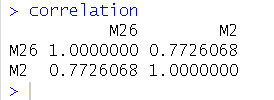
\includegraphics[width=10cm]{imagens/Resultado_Correlacao_Questao2.png}
    \caption{Output da correlação}
    \label{outputCorrelacaoQ2}
\end{figure}

\vspace{0.2cm}

\textbf{Conclusão:} O output da Figura \ref{outputCorrelacaoQ2} indica os coeficientes de correlação, que oscilam entre -1 e 1. Se for 1 é uma correlação perfeita positiva, enquanto que se for -1 é uma correlação perfeita negativa. Quanto mais próximo do 1 ou -1, maior é a correlação entre as duas varáveis. Por isso, chegamos à conclusão de que M2 e M26 têm um coeficiente de correlação de 0.77, o que indica que são consideravelmente correlacionadas.